In this Chapter we will get a closer look to the steps we took towards Socii implementation. First we will present a small proof of concept as mean for validation of our architectural main workflow (get the network rendered with OSN data), and at the same time experimenting with some technologies that we think that best suite our needs, we will then present our technological choices based on this first proof of concept.\\
\indent In the next parts of the Chapter, we will detail more on each component of our system from the extraction component to the front-end of Socii. We will also present at the end of the Chapter some of the main workflows within Socii and how all the components interact between them in order to produce a certain outcome.

%% ---------------------------------------------- Implementation first steps
\section{Implementation first steps}
In this section we describe our approach towards the implementation of the system, we will describe the process since the requirements
definition to the technological choices, some challenges and implementation details.

For gathering requirements we simply defined two groups, the first, the system Back-end has essential base functionalities, we focused only
on the essential without scoping or prioritizing, all the collected requirements are in the progress of being implemented, these include
web crawling modules, data mining for some data treatment and an extraction manager that allows remote calls of parameterized (granular) extractions.
In the system Front-end we followed a different approach by collecting a larger group of requirements that consist mainly in user interactions with the tool,
allowing us to narrow down the essential features based on requirements comparison. So at the end we sum up a few \textit{must have} requirements that
define the system identity an reflect the principles on which the project was designed upon (accessibility, simplicity, \glspl{osn} integration and contextual analysis).\\

\indent From here we built a simple \textit{proof of concept} that demonstrates the most basic of the workflow, this consists in a few steps that we next list:
\begin{itemize}
    \item \textbf{Back-end} - Extract users from a \gls{osn} (for this particular case we used Facebook as source);
    \item \textbf{Service Aggregator} - Aggregate the extracted users in a graph respecting front end data contract;
    \item \textbf{Front-end} - Rendering a graph on the browser, allow simple interaction of node data display on the user mouse click.
\end{itemize}

\subsection*{Aside note}
As one may noticed in the previous list, for sake of objectivity we skipped the implementation of some pieces in the architecture,
namely, the network metrics \gls{api} and the data mining process. In fact, these will only be included in the full implementation, because for the current proof
of concept we labeled this components as complements (this may be seen as add ons or plugins that added to proof of concept will bring the
project to life).\\

\subsection{Proof of concept results}
\indent The previously listed steps prove that the designed architecture produces the expected results, furthermore we also conclude in an empiric way what are the best tools and technologies that better suite the project requirements.\\

\begin{figure}[h!]
\begin{center}
  \hspace*{-0.8in}
  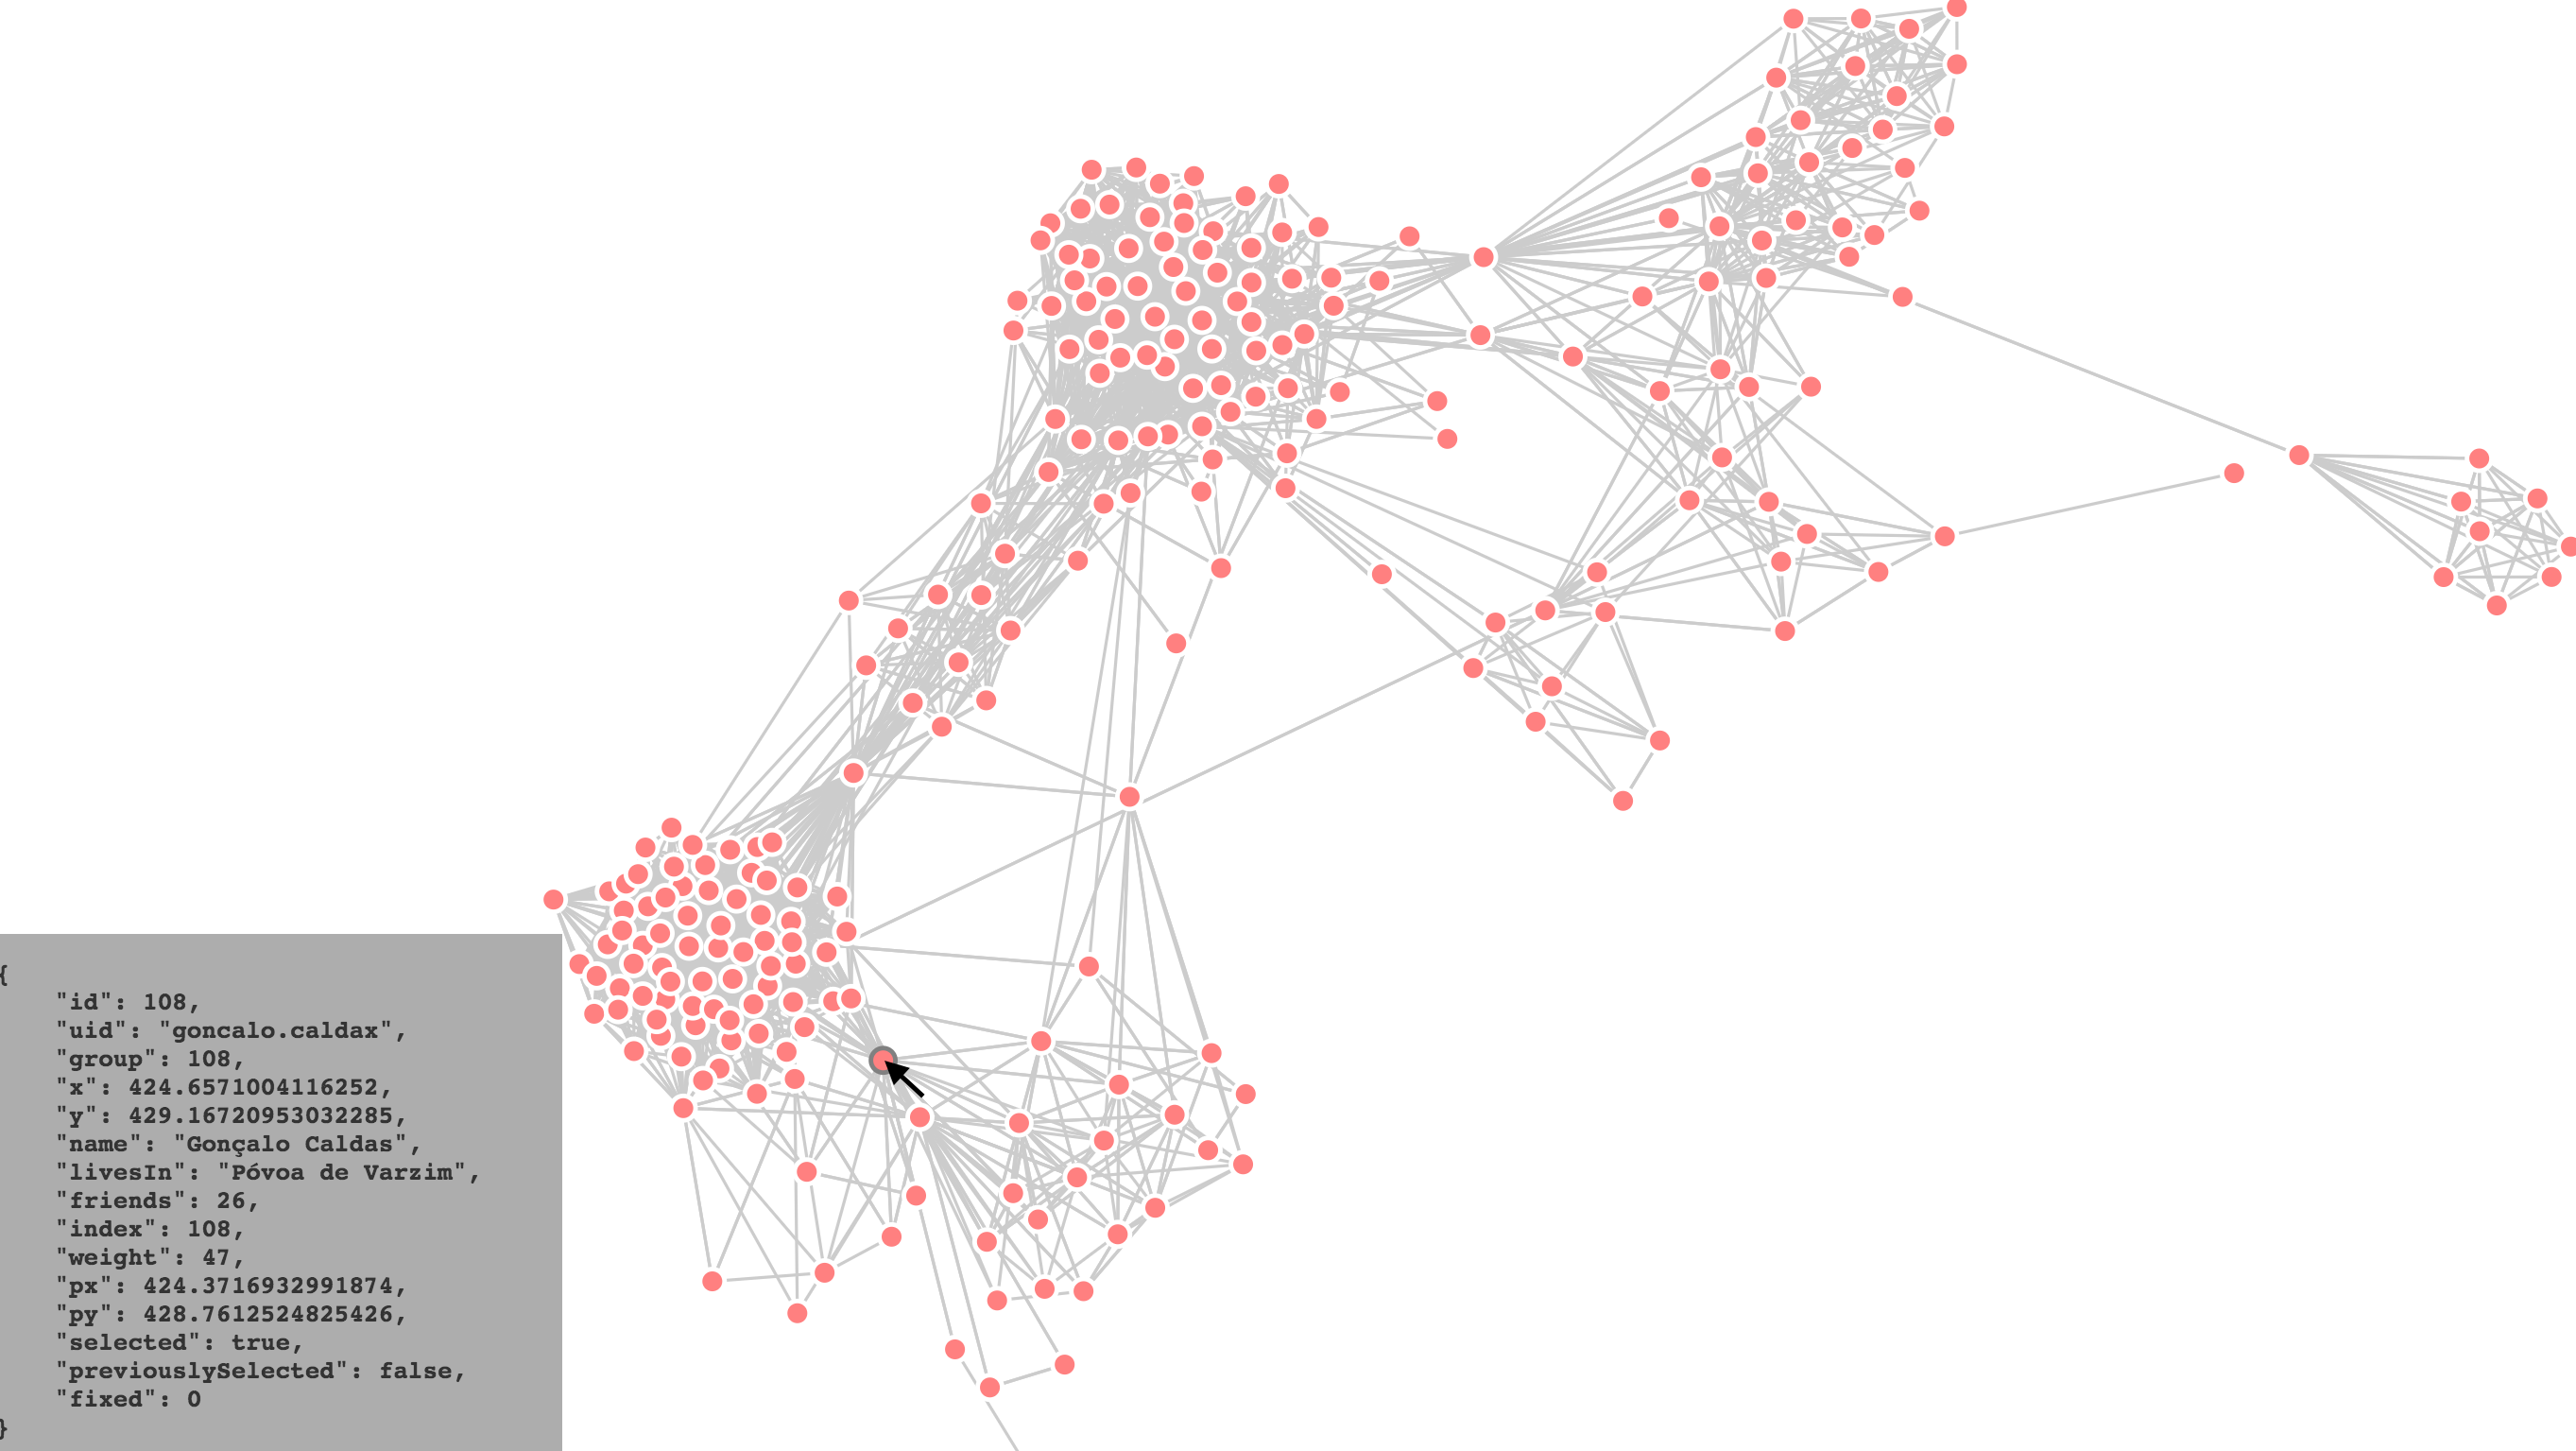
\includegraphics[width=1.2\textwidth]{img/proof-of-concept.png}
\end{center}
\caption{\label{img:poc} A \textit{screenshoot} of our first proof of concept.}
\end{figure}

\indent In Figure \ref{img:poc}, we can observe a network being rendered, this represents the friendship network of a given user. Since there is an entry point user, if we let him in this network we would obtain a egocentric network that could not depict all the surrounding relations in this small society. What we did was
to remove this node in order to obtain more clarity to observe the network. At Figure \ref{img:poc} we also can see the interaction of clicking on a certain node and displaying the node information.

\section{Choice of Technologies}
Having the requirements been defined and a small proof of concept been developed as we see in the previous section, we are now able to present our technological choices and provide some context on how we came to these conclusions. We will divide the presentation into four main sections where we present technologies specific to an application layer, starting from database technologies until we reach the front end technologies. For each section we first list the technologies and then we present the motives that lead us to that specific choices.

\subsection{Database technologies}
\begin{itemize}
    \item \textbf{MongoDB}.
\end{itemize}

Relational databases are one of the complex and advanced technologies that we have today. We have been building our applications on top of these technologies with very strict rules that allow our data to remain coherent through applications lifetimes. Databases engines such as MySQL, PostgreSQL and SQL Server are good live examples of the relevance of these technologies. Meanwhile, applications have grown not just in size but also in complexity, the \textit{web era} came, and with it the need for tools that allow us to manage unstructured data. Other alternatives to relational databases have emerged, today known as \textbf{non relational databases} (also known as NoSQL databases). These are database engines that allow us to store unstructured data or store data in a non relational way.\\
\indent We use \textbf{MongoDB} \citep{mongodb} (a document oriented database) to store data, this gives us more flexibility in manipulating complex JSON structures that are persisted in documents. These flexibility and interoperability would be considerably more complex to achieve using relational databases.

\subsection{Back-end technologies}
\begin{itemize}
    \item \textbf{Flask};
    \item \textbf{Python},
    \item \textbf{networkx};
    \item \textbf{PhantomJS};
    \item \textbf{Selenium WebDriver};
    \item \textbf{XPath}.
\end{itemize}

The main language that will support our back-end is \textbf{Python}. The choice for this language came very naturally since Python is one of the most used programming languages in the data science field along with others such as R or Java. We also choose Python for two other main reasons: first, we will be building data scrapper modules that need to simulate browser interactions.
 For that we will use \textbf{Selenium WebDriver} \citep{documentation2013selenium} for browser automation and interaction (with the complement of \textbf{PhantomJS} \citep{hidayat2013phantomjs}, a headless browser with a Javascript API), and Python integrates very naturally with these technologies, along side with \textbf{XPath} \citep{clark1999xml} for querying HTML pages and narrow extraction to the essentials; second because \textbf{networkx} \citep{hagberg2013networkx} that, already presented in Chapter 4, is written in Python and is a Python module. networkx is the most popular and powerful library that offers a large range of metrics and algorithms to run against graphs that come \textit{out of the box}.\\
\indent For networking, to make our back-end services available through web \glspl{api}, we will use \textbf{flask} \citep{ronacher2015flask}, a micro-framework for building simple networking applications in Python.

\subsection{Middleware technologies}
\begin{itemize}
    \item \textbf{NodeJS};
\end{itemize}

Sometimes we just need something very specific to perform some networking middleware operations, for this purpose NodeJS \citep{nodejs} is an emerging technology
that has been famous for performing well this kind of tasks. For bridging between our back-end and front-end we might need some small pieces that act
as \textit{glue} between these two larger components, we will use NodeJS for that purpose.

\subsection{Front-end technologies}
\begin{itemize}
    \item \textbf{HTML};
    \item \textbf{Javascript};
    \item \textbf{CSS};
    \item \textbf{D3.js};
    \item \textbf{React};
\end{itemize}

Since we are building a web application, we automatically address to three main technologies that need no introduction, these are HTML, Javascript and CSS. In complement, we will use for our specific needs, that consist in building interactive graphs, a web data driven document representation system, \textbf{D3.js} \citep{bostock2012d3}. In what concerns to visualization D3.js will be our main third party, that will bring us many features to help us on network representation and graph interaction \footnote{in our proof of concept we already used D3.js for rendering the network as we have demonstrated in Figure \ref{img:poc}}.
In order to improve our application performance and also the development process, we choose a modern web library, React \citep{react}.

%% ---------------------------------------------- Implementation details
\section{Implementation details}

In this section we will explain with more detail the more important parts of the system, how they were implemented with some technical notes and more importantly how they interact within our architecture. We show some of the main workflows of the Socii tool in order to clarify that.

\subsection{Extraction (web crawlers)}
The web crawler is the module that will allow us to extract data from \glspl{osn}. Each \gls{osn} has its own web site so each web crawler module has its own implementation, still the extract operations are wrapped in a single API as we described in Chapter 6 when explaining the requirements for the web crawlers. The workflow for extracting some user is the following:
\begin{itemize}
    \item Login with user credentials;
    \item Go to a specific page within its social profile;
    \item Perform extraction on that page.
\end{itemize}
These listed three steps may be repeated more than one time since we extract information from different pages. In the following explanations we will be referring to Facebook implementation details for clarification only.

\subsubsection*{Login}
This piece of code performs the login:

\lstinputlisting[language=Python]{code/login.py}

Here we see that browser driver is used to navigate between pages and selector functions such as \textit{find\_element\_by\_id} (line 8 to 10) are used to access DOM elements.

\subsubsection*{Perform extraction of facebook friends list}
The following function extracts a list of Facebook friends:

\lstinputlisting[language=Python]{code/facebook_friends_list.py}

Here we see some helper functions where the names are sufficiently explicit in order for one to understand the goal of this function without consulting the others. First we navigate to the users' friends list, then we get the total number of friends and call \textbf{\_load\_all\_friends} (line 7) that will scroll the friends' list in order to load all friends in the same page (this needs to happen because Facebook uses lazy loading of friends in order to not load them at once in the web page). Next we get the container that wraps the friends list (line 9), loop for each block that holds some friend info (line 12) and for each one of them we extract the \textbf{user id (uid)} from the link to the friend's profile, this may be a numeric value (line 16) (code in the \textit{try} block) or it can be a string that comes as first parameters in the URL query (line 20) (\textit{except} block).

\subsection{Network generator}

Network generator is a very purpose-oriented piece of software in this architecture. Its only goal is to produce data sets (users) for a given \gls{osn}. This component is implemented in \textit{Node JS} and it uses faker \citep{fakerjs} in order to generate data for a given data schema. Next we show a simple schema for Facebook data generator.

\lstinputlisting[language=java]{code/fb_schema.js}

We also add some threshold restriction to some values in order to not produce extremely unrealistic data.

\lstinputlisting[language=java]{code/fb_restrict.js}

Given a data model and a set of restrictions we generate sets of contextualized data for a given \gls{osn} (in the previous examples, for Facebook).

\subsection{Network metrics}
As we mentioned already in this Chapter (Section 7.2) we use networkx \citep{hagberg2013networkx} to perform metrics calculations such as centrality measures (betweenness, degree, eigenvector etc.), node rank or clustering against a network that is fed into this API. This micro service is very simple and could practically be seen as a wrapper to networkx methods. In the API we made available an endpoint \textbf{/metrics} that is available to receive metrics requests. Below a sample payload that the \textbf{/metrics} endpoint is expecting in order to calculate metrics.

\lstinputlisting[language=java]{code/metrics_payload.js}

If no metrics array is requested all metrics will be computed, this is a fallback/default API behavior.\\
\indent The response is a mapping between each node and the respective computed metrics, and a \textbf{global} object that holds metrics for the graph.

\lstinputlisting[language=java]{code/metrics_response.js}

Next we present the piece of code responsible for receiving such request and bridge it with the networkx software wrapper module (our \textbf{nx\_interface}). The responsibility for computing the metrics is delegated to the \textbf{nx\_interface} which calls the correct networkx method for computing a given metric.

\lstinputlisting[language=Python]{code/metrics_api.py}

Then we simply observe what are the requested metrics and build a response that is divided into two metrics groups. \textbf{Node} metrics are node specific, meaning that we will have this metric value for each node; other metrics are global, these are metrics that concern to the network as a global entity (e.g. network clustering coefficient). The next presented method is called one time per metric.

\lstinputlisting[language=Python]{code/nx_interface.py}

\subsection{Service Aggregator}
Anytime our front end needs to interact with some of the previous micro services, it goes through this service aggregator
in order to fetch data or to perform some other data operation. This service aggregator also manages Socii users concerning the authentication process.
Next we present a simple generic client that is implemented in our aggregator in order to communicate with the metrics micro service.

\lstinputlisting[language=java]{code/metrics_client.js}

In the Section 7.4 we will explain the main workflow that takes place inside the service aggregator, and there more details about this component will be provided.

\subsubsection{Middleware optimizations}
Some optimizations were put in place considering that this is the main networking component, where more traffic flows. The considered optimizations consist in using an existent middleware third parties in order to mitigate high payload exchange (between front-end and aggregator, and also between aggregator and other micro services). We use the \textbf{compression} \footnote{\url{https://github.com/expressjs/compression}} NodeJs middleware to achieve optimal payload compression levels.

\subsection{Front-end}

Our front-end is built using the react library as we have already mentioned, and the main component of the application consists on a visualization dashboard that displays an interactive network that is rendered using an open source component that we have built, \textbf{react-d3-graph} \citep{reactd3graph} that will be explained in the following sections. Other relevant third parties that we use in our front end are the following:

\begin{itemize}
    \item \textit{\textbf{react-redux}}\footnote{Official React bindings for Redux \url{https://github.com/reactjs/react-redux}} - redux architecture official bindings for React library. This eases the process of manage application state.
    \item \textit{\textbf{axios}}\footnote{Promise based HTTP client for the browser and node.js \url{https://github.com/mzabriskie/axios}} - an HTTP client library that makes networking operations more straightforward.
    \item \textit{\textbf{material-ui}} \footnote{React Components that Implement Google's Material Design \url{http://www.material-ui.com}} - a library that offers visual components with a pre established look and feel and some built in interactions.
    \item \textit{\textbf{react-bootstrap}} \footnote{Bootstrap 3 components built with React \url{https://react-bootstrap.github.io/}} - a complement to the previous library, this one offers also some visual components like overlays and tooltips.
\end{itemize}

\subsubsection{Graph render and interaction component with react-d3-graph}

\begin{quote}
\textit{"React component to build interactive and configurable graphs with d3 effortlessly"}
\end{quote}

From an end user perspective the most relevant and valuable aspects of a \gls{sna} tool are powerful network interactions and clean visualization (and by clean we mean perceptible). In order to achieve this in Socii our efforts were directed into a generic, reusable and configurable software: \textbf{react-d3-graph} \citep{reactd3graph}. This component allows us to focus only on the visualization features and in how we want to represent and interact with our network (graph). This component is built on top of the react library and creates configurable abstractions upon D3.js. All the detailed documentation \footnote{\url{https://danielcaldas.github.io/react-d3-graph/docs/index.html}} of react-d3-graph
may be consulted on the web, also a live demo\footnote{\url{https://danielcaldas.github.io/react-d3-graph/sandbox/index.html}} with the all the possible public configurations offered by react-d3-graph is also available.\\
With this development we will isolate all the visualization concerns leaving Socii with less work on this matter. Also Socii can wrap this component and use the available user actions to interact with the graph, and all the visual aspects such as nodes colors or text size may or may not be editable by a Socii user. Socii has the power to decide the level of granularity of user control upon graph configurations, but of course since we want a simple application we will leave to Socii how the network looks like exposing some basic interactions to the end user such as node click, zooming, mouse overing and drag and drop on all the network or upon a specific node.

%% ---------------------------------------------- Main Workflows
\section{Main Workflows}

In this section we describe two of our main workflows within Socii tool. The first and most relevant workflow is the network aggregation and rendering that has within its main intervenient the aggregator. Next sections clarify the role of this aggregator. Then we will present a front-end only interaction that consists in coloring nodes with given properties.

\subsubsection{Network Aggregation and Rendering}

\begin{figure}[h!]
\begin{center}
  \hspace*{-0.8in}
  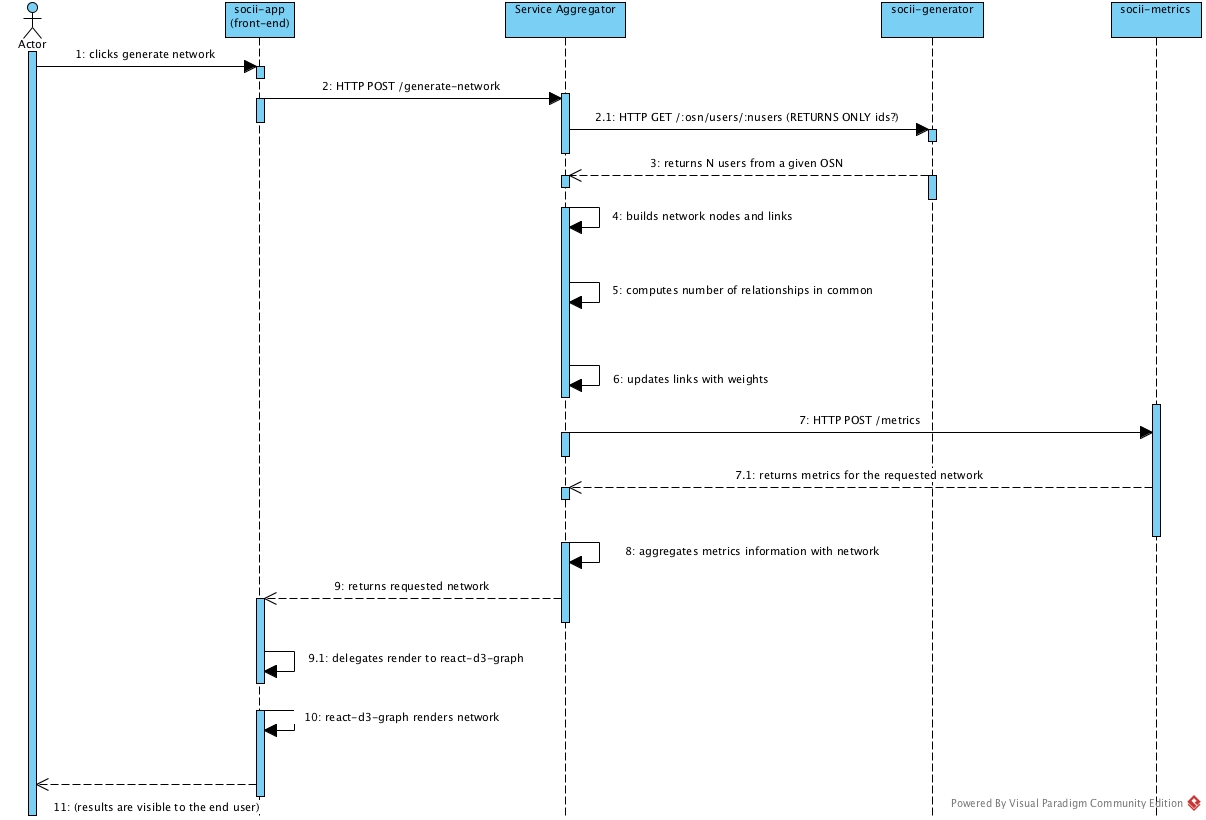
\includegraphics[width=1.2\textwidth]{img/socii-sd.jpg}
\end{center}
\caption{\label{img:sociisd} In this figure we may observe Socii sequence diagram for building a network.}
\end{figure}

In the diagram of Figure \ref{img:sociisd}, one may observe what happens since the user requests that a certain \gls{osn} network is built. In the next explanation we will be referring to the workflow steps numbers in the figure.\\
\indent First the user configures the network choosing the number of nodes for a certain \gls{osn} and what metrics he wants to calculate against the network and then see in the network visualizer area. Then the user presses a button that orders network build (\textbf{1}, \textbf{2}), and waits until all the aggregation operations are performed.\\
\indent First the service aggregator fetches a set of \textit{N} requested users from the \textbf{socii-generator} (\textbf{2.1}) microservice, then based on the retrieved information it builds the network nodes and links data structure and performs some other minor operations (\textbf{4,5,6}). Once the previous operations are completed a request is made to the \textbf{socii-metrics} microservice in order to collect the metrics for the previous built network. The returned metric values are aggregated with the users, nodes and links within a network data structure (\textbf{8}) and a response is sent to the front-end (\textbf{9}). The front-end only needs to take the nodes and links that the aggregator puts together and delegate the network rendering to the react-d3-graph component (\textbf{10}), and that's it, the user has now available the full network with all the aggregated information (\textbf{11}).

\subsubsection{Community detection with node coloring by property}

In this case we present a more simple workflow that happens only on the front-end. The community detection is a module that allows the user to paint nodes that have some property in common. For example, lets say we want to color our network according to where the users live, we will have to associate a unique color per city and then map these colors to the nodes painting each node with the color that corresponds to the corresponding user's city. This algorithm is generic so we can reproduce the same of other properties such as birthday, name or gender.

\begin{figure}[h!]
\begin{center}
  \hspace*{-0.8in}
  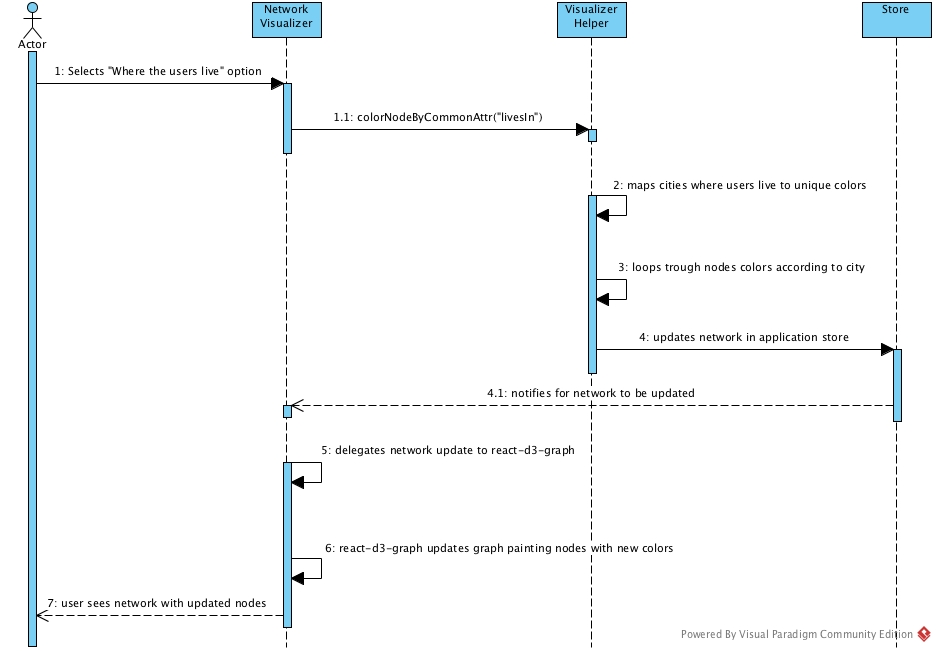
\includegraphics[width=1.2\textwidth]{img/socii-cdet.jpg}
\end{center}
\caption{\label{img:sociicdet} Socii sequence diagram community detection based on node properties.}
\end{figure}

As we can see in Figure \ref{img:sociicdet} the process is simple, the user chooses an available property for community detection (\textbf{1}), then some logic helper front-end component takes the request and maps the different cities to a unique color (\textbf{2}). The next step consists in painting user nodes according to the color of their city (\textbf{3}) and update the store (the store is the object that holds the network state, this includes nodes and their properties). When the store is updated the network visualizer component is notified and delegates the new node properties to react-d3-graph that handles visual updates (\textbf{5 and 6}).
